\documentclass[a4paper,12pt]{article}
\usepackage[margin=18mm]{geometry}
\usepackage{tikz}
\usepackage{amsmath}
\newcommand{\pFourCell}[2]{\makebox[#1em][c]{\ensuremath{#2}}}
\pagestyle{empty}
\begin{document}
\section*{Spaltentreue LaTeX-Ausgabe}
\noindent Gleichung: \texttt{sin(sqrt((x+3)/(2+1)))=5} \hfill Zielvariable: \texttt{x} \hfill Profil: \texttt{standard}

\vspace{8mm}
\begin{center}
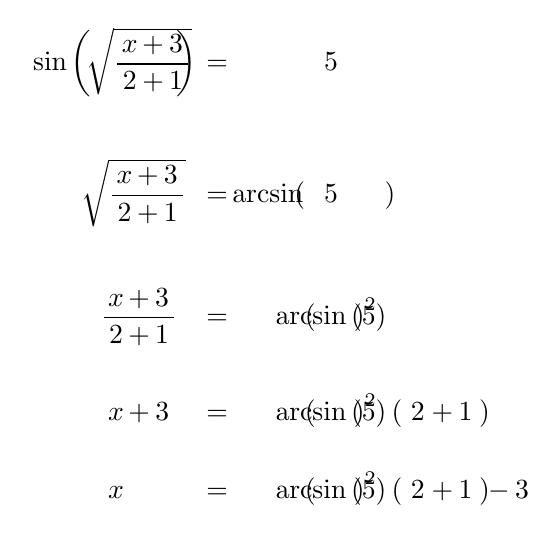
\begin{tikzpicture}[x=1em,y=-1em]
\node[anchor=base, inner sep=0pt] at (4.02,2.9) {$\pFourCell{2.56}{\sqrt{\displaystyle\frac{\pFourCell{0.9}{x}\pFourCell{0.78}{+}\pFourCell{0.88}{3}}{\pFourCell{0.9}{2}\pFourCell{0.78}{+}\pFourCell{0.88}{1}}}}$};
\node[anchor=base, inner sep=0pt] at (0.81,2.9) {$\pFourCell{1.62}{\sin}$};
\node[anchor=base, inner sep=0pt] at (1.99,2.9) {$\pFourCell{0.74}{\left(\vphantom{\pFourCell{2.56}{\sqrt{\displaystyle\frac{\pFourCell{0.9}{x}\pFourCell{0.78}{+}\pFourCell{0.88}{3}}{\pFourCell{0.9}{2}\pFourCell{0.78}{+}\pFourCell{0.88}{1}}}}}\right.}$};
\node[anchor=base, inner sep=0pt] at (5.67,2.9) {$\pFourCell{0.74}{\left.\vphantom{\pFourCell{2.56}{\sqrt{\displaystyle\frac{\pFourCell{0.9}{x}\pFourCell{0.78}{+}\pFourCell{0.88}{3}}{\pFourCell{0.9}{2}\pFourCell{0.78}{+}\pFourCell{0.88}{1}}}}}\right)}$};
\node[anchor=base, inner sep=0pt] at (6.85,2.9) {$=$};
\node[anchor=base, inner sep=0pt] at (10.96,2.9) {$5$};
\node[anchor=base, inner sep=0pt] at (3.83,7.65) {$\pFourCell{2.94}{\sqrt{\displaystyle\frac{\pFourCell{0.9}{x}\pFourCell{0.78}{+}\pFourCell{0.88}{3}}{\pFourCell{0.9}{2}\pFourCell{0.78}{+}\pFourCell{0.88}{1}}}}$};
\node[anchor=base, inner sep=0pt] at (6.85,7.65) {$=$};
\node[anchor=base, inner sep=0pt] at (10.96,7.65) {$\pFourCell{1}{5}$};
\node[anchor=base, inner sep=0pt] at (8.68,7.65) {$\pFourCell{2.04}{\arcsin}$};
\node[anchor=base, inner sep=0pt] at (9.89,7.65) {$\pFourCell{0.38}{\left(\vphantom{\pFourCell{1}{5}}\right.}$};
\node[anchor=base, inner sep=0pt] at (13.03,7.65) {$\pFourCell{0.38}{\left.\vphantom{\pFourCell{1}{5}}\right)}$};
\node[anchor=base, inner sep=0pt] at (4.02,12.075) {$\displaystyle\frac{\pFourCell{0.9}{x}\pFourCell{0.78}{+}\pFourCell{0.88}{3}}{\pFourCell{0.9}{2}\pFourCell{0.78}{+}\pFourCell{0.88}{1}}$};
\node[anchor=base, inner sep=0pt] at (6.85,12.075) {$=$};
\node[anchor=base, inner sep=0pt] at (10.96,12.075) {$\pFourCell{1}{\arcsin\left(5\right)}$};
\node[anchor=base, inner sep=0pt] at (10.27,12.075) {$\pFourCell{0.38}{\left(\vphantom{\pFourCell{1}{\arcsin\left(5\right)}}\right.}$};
\node[anchor=base, inner sep=0pt] at (12.15,12.075) {$\pFourCell{1.38}{\left.\vphantom{\pFourCell{1}{\arcsin\left(5\right)}}\right)^{2}}$};
\node[anchor=base, inner sep=0pt] at (3.19,15.535) {$x$};
\node[anchor=base, inner sep=0pt] at (4.03,15.535) {$+$};
\node[anchor=base, inner sep=0pt] at (4.86,15.535) {$3$};
\node[anchor=base, inner sep=0pt] at (6.85,15.535) {$=$};
\node[anchor=base, inner sep=0pt] at (10.96,15.535) {$\pFourCell{1}{\arcsin\left(5\right)}$};
\node[anchor=base, inner sep=0pt] at (10.27,15.535) {$\pFourCell{0.38}{\left(\vphantom{\pFourCell{1}{\arcsin\left(5\right)}}\right.}$};
\node[anchor=base, inner sep=0pt] at (12.15,15.535) {$\pFourCell{1.38}{\left.\vphantom{\pFourCell{1}{\arcsin\left(5\right)}}\right)^{2}}$};
\node[anchor=base, inner sep=0pt] at (14.93,15.535) {$\pFourCell{1}{2}\pFourCell{0.78}{+}\pFourCell{0.88}{1}$};
\node[anchor=base, inner sep=0pt] at (13.41,15.535) {$\pFourCell{0.38}{\left(\vphantom{\pFourCell{1}{2}\pFourCell{0.78}{+}\pFourCell{0.88}{1}}\right.}$};
\node[anchor=base, inner sep=0pt] at (16.45,15.535) {$\pFourCell{0.38}{\left.\vphantom{\pFourCell{1}{2}\pFourCell{0.78}{+}\pFourCell{0.88}{1}}\right)}$};
\node[anchor=base, inner sep=0pt] at (3.19,18.355) {$x$};
\node[anchor=base, inner sep=0pt] at (6.85,18.355) {$=$};
\node[anchor=base, inner sep=0pt] at (10.96,18.355) {$\pFourCell{1}{\arcsin\left(5\right)}$};
\node[anchor=base, inner sep=0pt] at (10.27,18.355) {$\pFourCell{0.38}{\left(\vphantom{\pFourCell{1}{\arcsin\left(5\right)}}\right.}$};
\node[anchor=base, inner sep=0pt] at (12.15,18.355) {$\pFourCell{1.38}{\left.\vphantom{\pFourCell{1}{\arcsin\left(5\right)}}\right)^{2}}$};
\node[anchor=base, inner sep=0pt] at (14.93,18.355) {$\pFourCell{1}{2}\pFourCell{0.78}{+}\pFourCell{0.88}{1}$};
\node[anchor=base, inner sep=0pt] at (13.41,18.355) {$\pFourCell{0.38}{\left(\vphantom{\pFourCell{1}{2}\pFourCell{0.78}{+}\pFourCell{0.88}{1}}\right.}$};
\node[anchor=base, inner sep=0pt] at (16.45,18.355) {$\pFourCell{0.38}{\left.\vphantom{\pFourCell{1}{2}\pFourCell{0.78}{+}\pFourCell{0.88}{1}}\right)}$};
\node[anchor=base, inner sep=0pt] at (17.03,18.355) {$-$};
\node[anchor=base, inner sep=0pt] at (17.86,18.355) {$3$};
\end{tikzpicture}
\end{center}

\newpage
\section*{Spaltentreue LaTeX-Ausgabe mit Spaltengrenzen}
\vspace{6mm}
\begin{center}
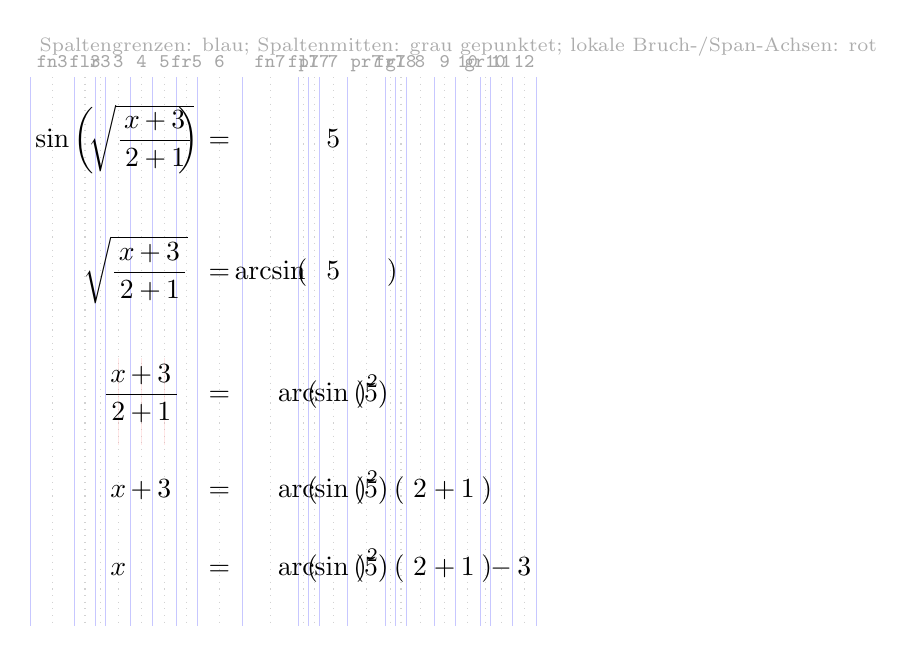
\begin{tikzpicture}[x=1em,y=-1em]
\node[font={\scriptsize}, text=gray!65, anchor=west] at (0,-0.75) {Spaltengrenzen: blau; Spaltenmitten: grau gepunktet; lokale Bruch-/Span-Achsen: rot};
\draw[blue!22, line width=0.28pt] (0,0.35) -- (0,20.19);
\draw[blue!22, line width=0.28pt] (1.62,0.35) -- (1.62,20.19);
\draw[blue!22, line width=0.28pt] (2.36,0.35) -- (2.36,20.19);
\draw[blue!22, line width=0.28pt] (2.74,0.35) -- (2.74,20.19);
\draw[blue!22, line width=0.28pt] (3.64,0.35) -- (3.64,20.19);
\draw[blue!22, line width=0.28pt] (4.42,0.35) -- (4.42,20.19);
\draw[blue!22, line width=0.28pt] (5.3,0.35) -- (5.3,20.19);
\draw[blue!22, line width=0.28pt] (6.04,0.35) -- (6.04,20.19);
\draw[blue!22, line width=0.28pt] (7.66,0.35) -- (7.66,20.19);
\draw[blue!22, line width=0.28pt] (9.7,0.35) -- (9.7,20.19);
\draw[blue!22, line width=0.28pt] (10.08,0.35) -- (10.08,20.19);
\draw[blue!22, line width=0.28pt] (10.46,0.35) -- (10.46,20.19);
\draw[blue!22, line width=0.28pt] (11.46,0.35) -- (11.46,20.19);
\draw[blue!22, line width=0.28pt] (12.84,0.35) -- (12.84,20.19);
\draw[blue!22, line width=0.28pt] (13.22,0.35) -- (13.22,20.19);
\draw[blue!22, line width=0.28pt] (13.6,0.35) -- (13.6,20.19);
\draw[blue!22, line width=0.28pt] (14.6,0.35) -- (14.6,20.19);
\draw[blue!22, line width=0.28pt] (15.38,0.35) -- (15.38,20.19);
\draw[blue!22, line width=0.28pt] (16.26,0.35) -- (16.26,20.19);
\draw[blue!22, line width=0.28pt] (16.64,0.35) -- (16.64,20.19);
\draw[blue!22, line width=0.28pt] (17.42,0.35) -- (17.42,20.19);
\draw[blue!22, line width=0.28pt] (18.3,0.35) -- (18.3,20.19);
\draw[gray!35, dotted] (0.81,0.35) -- (0.81,20.19);
\node[font={\ttfamily\scriptsize}, text=gray!70, anchor=base] at (0.81,0) {fn3};
\draw[gray!35, dotted] (1.99,0.35) -- (1.99,20.19);
\node[font={\ttfamily\scriptsize}, text=gray!70, anchor=base] at (1.99,0) {fl3};
\draw[gray!35, dotted] (2.55,0.35) -- (2.55,20.19);
\node[font={\ttfamily\scriptsize}, text=gray!70, anchor=base] at (2.55,0) {r3};
\draw[gray!35, dotted] (3.19,0.35) -- (3.19,20.19);
\node[font={\ttfamily\scriptsize}, text=gray!70, anchor=base] at (3.19,0) {3};
\draw[gray!35, dotted] (4.03,0.35) -- (4.03,20.19);
\node[font={\ttfamily\scriptsize}, text=gray!70, anchor=base] at (4.03,0) {4};
\draw[gray!35, dotted] (4.86,0.35) -- (4.86,20.19);
\node[font={\ttfamily\scriptsize}, text=gray!70, anchor=base] at (4.86,0) {5};
\draw[gray!35, dotted] (5.67,0.35) -- (5.67,20.19);
\node[font={\ttfamily\scriptsize}, text=gray!70, anchor=base] at (5.67,0) {fr5};
\draw[gray!35, dotted] (6.85,0.35) -- (6.85,20.19);
\node[font={\ttfamily\scriptsize}, text=gray!70, anchor=base] at (6.85,0) {6};
\draw[gray!35, dotted] (8.68,0.35) -- (8.68,20.19);
\node[font={\ttfamily\scriptsize}, text=gray!70, anchor=base] at (8.68,0) {fn7};
\draw[gray!35, dotted] (9.89,0.35) -- (9.89,20.19);
\node[font={\ttfamily\scriptsize}, text=gray!70, anchor=base] at (9.89,0) {fl7};
\draw[gray!35, dotted] (10.27,0.35) -- (10.27,20.19);
\node[font={\ttfamily\scriptsize}, text=gray!70, anchor=base] at (10.27,0) {pl7};
\draw[gray!35, dotted] (10.96,0.35) -- (10.96,20.19);
\node[font={\ttfamily\scriptsize}, text=gray!70, anchor=base] at (10.96,0) {7};
\draw[gray!35, dotted] (12.15,0.35) -- (12.15,20.19);
\node[font={\ttfamily\scriptsize}, text=gray!70, anchor=base] at (12.15,0) {pr7};
\draw[gray!35, dotted] (13.03,0.35) -- (13.03,20.19);
\node[font={\ttfamily\scriptsize}, text=gray!70, anchor=base] at (13.03,0) {fr7};
\draw[gray!35, dotted] (13.41,0.35) -- (13.41,20.19);
\node[font={\ttfamily\scriptsize}, text=gray!70, anchor=base] at (13.41,0) {gl8};
\draw[gray!35, dotted] (14.1,0.35) -- (14.1,20.19);
\node[font={\ttfamily\scriptsize}, text=gray!70, anchor=base] at (14.1,0) {8};
\draw[gray!35, dotted] (14.99,0.35) -- (14.99,20.19);
\node[font={\ttfamily\scriptsize}, text=gray!70, anchor=base] at (14.99,0) {9};
\draw[gray!35, dotted] (15.82,0.35) -- (15.82,20.19);
\node[font={\ttfamily\scriptsize}, text=gray!70, anchor=base] at (15.82,0) {10};
\draw[gray!35, dotted] (16.45,0.35) -- (16.45,20.19);
\node[font={\ttfamily\scriptsize}, text=gray!70, anchor=base] at (16.45,0) {gr10};
\draw[gray!35, dotted] (17.03,0.35) -- (17.03,20.19);
\node[font={\ttfamily\scriptsize}, text=gray!70, anchor=base] at (17.03,0) {11};
\draw[gray!35, dotted] (17.86,0.35) -- (17.86,20.19);
\node[font={\ttfamily\scriptsize}, text=gray!70, anchor=base] at (17.86,0) {12};
\node[anchor=base, inner sep=0pt] at (4.02,2.9) {$\pFourCell{2.56}{\sqrt{\displaystyle\frac{\pFourCell{0.9}{x}\pFourCell{0.78}{+}\pFourCell{0.88}{3}}{\pFourCell{0.9}{2}\pFourCell{0.78}{+}\pFourCell{0.88}{1}}}}$};
\node[anchor=base, inner sep=0pt] at (0.81,2.9) {$\pFourCell{1.62}{\sin}$};
\node[anchor=base, inner sep=0pt] at (1.99,2.9) {$\pFourCell{0.74}{\left(\vphantom{\pFourCell{2.56}{\sqrt{\displaystyle\frac{\pFourCell{0.9}{x}\pFourCell{0.78}{+}\pFourCell{0.88}{3}}{\pFourCell{0.9}{2}\pFourCell{0.78}{+}\pFourCell{0.88}{1}}}}}\right.}$};
\node[anchor=base, inner sep=0pt] at (5.67,2.9) {$\pFourCell{0.74}{\left.\vphantom{\pFourCell{2.56}{\sqrt{\displaystyle\frac{\pFourCell{0.9}{x}\pFourCell{0.78}{+}\pFourCell{0.88}{3}}{\pFourCell{0.9}{2}\pFourCell{0.78}{+}\pFourCell{0.88}{1}}}}}\right)}$};
\node[anchor=base, inner sep=0pt] at (6.85,2.9) {$=$};
\node[anchor=base, inner sep=0pt] at (10.96,2.9) {$5$};
\node[anchor=base, inner sep=0pt] at (3.83,7.65) {$\pFourCell{2.94}{\sqrt{\displaystyle\frac{\pFourCell{0.9}{x}\pFourCell{0.78}{+}\pFourCell{0.88}{3}}{\pFourCell{0.9}{2}\pFourCell{0.78}{+}\pFourCell{0.88}{1}}}}$};
\node[anchor=base, inner sep=0pt] at (6.85,7.65) {$=$};
\node[anchor=base, inner sep=0pt] at (10.96,7.65) {$\pFourCell{1}{5}$};
\node[anchor=base, inner sep=0pt] at (8.68,7.65) {$\pFourCell{2.04}{\arcsin}$};
\node[anchor=base, inner sep=0pt] at (9.89,7.65) {$\pFourCell{0.38}{\left(\vphantom{\pFourCell{1}{5}}\right.}$};
\node[anchor=base, inner sep=0pt] at (13.03,7.65) {$\pFourCell{0.38}{\left.\vphantom{\pFourCell{1}{5}}\right)}$};
\draw[red!30, opacity=0.32, line width=0.35pt] (3.19,10.5) -- (3.19,13.65);
\draw[red!30, opacity=0.32, line width=0.35pt] (4.03,10.5) -- (4.03,13.65);
\draw[red!30, opacity=0.32, line width=0.35pt] (4.86,10.5) -- (4.86,13.65);
\node[anchor=base, inner sep=0pt] at (4.02,12.075) {$\displaystyle\frac{\pFourCell{0.9}{x}\pFourCell{0.78}{+}\pFourCell{0.88}{3}}{\pFourCell{0.9}{2}\pFourCell{0.78}{+}\pFourCell{0.88}{1}}$};
\node[anchor=base, inner sep=0pt] at (6.85,12.075) {$=$};
\node[anchor=base, inner sep=0pt] at (10.96,12.075) {$\pFourCell{1}{\arcsin\left(5\right)}$};
\node[anchor=base, inner sep=0pt] at (10.27,12.075) {$\pFourCell{0.38}{\left(\vphantom{\pFourCell{1}{\arcsin\left(5\right)}}\right.}$};
\node[anchor=base, inner sep=0pt] at (12.15,12.075) {$\pFourCell{1.38}{\left.\vphantom{\pFourCell{1}{\arcsin\left(5\right)}}\right)^{2}}$};
\node[anchor=base, inner sep=0pt] at (3.19,15.535) {$x$};
\node[anchor=base, inner sep=0pt] at (4.03,15.535) {$+$};
\node[anchor=base, inner sep=0pt] at (4.86,15.535) {$3$};
\node[anchor=base, inner sep=0pt] at (6.85,15.535) {$=$};
\node[anchor=base, inner sep=0pt] at (10.96,15.535) {$\pFourCell{1}{\arcsin\left(5\right)}$};
\node[anchor=base, inner sep=0pt] at (10.27,15.535) {$\pFourCell{0.38}{\left(\vphantom{\pFourCell{1}{\arcsin\left(5\right)}}\right.}$};
\node[anchor=base, inner sep=0pt] at (12.15,15.535) {$\pFourCell{1.38}{\left.\vphantom{\pFourCell{1}{\arcsin\left(5\right)}}\right)^{2}}$};
\node[anchor=base, inner sep=0pt] at (14.93,15.535) {$\pFourCell{1}{2}\pFourCell{0.78}{+}\pFourCell{0.88}{1}$};
\node[anchor=base, inner sep=0pt] at (13.41,15.535) {$\pFourCell{0.38}{\left(\vphantom{\pFourCell{1}{2}\pFourCell{0.78}{+}\pFourCell{0.88}{1}}\right.}$};
\node[anchor=base, inner sep=0pt] at (16.45,15.535) {$\pFourCell{0.38}{\left.\vphantom{\pFourCell{1}{2}\pFourCell{0.78}{+}\pFourCell{0.88}{1}}\right)}$};
\node[anchor=base, inner sep=0pt] at (3.19,18.355) {$x$};
\node[anchor=base, inner sep=0pt] at (6.85,18.355) {$=$};
\node[anchor=base, inner sep=0pt] at (10.96,18.355) {$\pFourCell{1}{\arcsin\left(5\right)}$};
\node[anchor=base, inner sep=0pt] at (10.27,18.355) {$\pFourCell{0.38}{\left(\vphantom{\pFourCell{1}{\arcsin\left(5\right)}}\right.}$};
\node[anchor=base, inner sep=0pt] at (12.15,18.355) {$\pFourCell{1.38}{\left.\vphantom{\pFourCell{1}{\arcsin\left(5\right)}}\right)^{2}}$};
\node[anchor=base, inner sep=0pt] at (14.93,18.355) {$\pFourCell{1}{2}\pFourCell{0.78}{+}\pFourCell{0.88}{1}$};
\node[anchor=base, inner sep=0pt] at (13.41,18.355) {$\pFourCell{0.38}{\left(\vphantom{\pFourCell{1}{2}\pFourCell{0.78}{+}\pFourCell{0.88}{1}}\right.}$};
\node[anchor=base, inner sep=0pt] at (16.45,18.355) {$\pFourCell{0.38}{\left.\vphantom{\pFourCell{1}{2}\pFourCell{0.78}{+}\pFourCell{0.88}{1}}\right)}$};
\node[anchor=base, inner sep=0pt] at (17.03,18.355) {$-$};
\node[anchor=base, inner sep=0pt] at (17.86,18.355) {$3$};
\end{tikzpicture}
\end{center}
\end{document}
